\chapter{\ifenglish Background Knowledge and Theory\else ทฤษฎีที่เกี่ยวข้อง\fi}

การทำโครงงาน เริ่มต้นด้วยการศึกษาค้นคว้า ทฤษฎีที่เกี่ยวข้อง หรือ งานวิจัย/โครงงาน ที่เคยมีผู้นำเสนอไว้แล้ว ซึ่งเนื้อหาในบทนี้ก็จะเกี่ยวกับการอธิบายถึงสิ่งที่เกี่ยวข้องกับโครงงาน เพื่อให้ผู้อ่านเข้าใจเนื้อหาในบทถัดๆ ไปได้ง่ายขึ้น

\section{เกมสยองขวัญแบบผู้เล่นหลายคนในตลาด}
\subsection{Dead Space 3}

Dead Space 3 เป็นเกมสยองขวัญที่ให้ผู้เล่นสามารถเล่นโดยใช้ความร่วมมือจากผู้เล่น 2 คน โดยต่อสู้กับ Necromorph โดยรวมแล้วเป็นเกมสยองขวัญเอาชีวิตรอดที่ตึงเครียดและน่าตื่นเต้นที่นำเสนอประสบการณ์ความร่วมมือที่สมจริง เรื่องราวที่น่าดึงดูด และกลไกการเล่นเกมที่หลากหลายเพื่อให้ผู้เล่นมีส่วนร่วมและลุ้นตาม \cite{DeadSpace3}

\begin{figure}[h]
  \begin{center}
  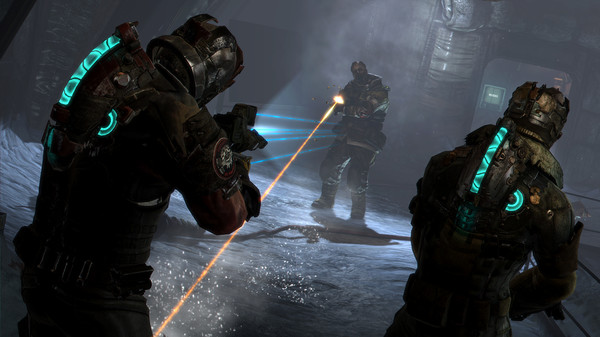
\includegraphics[width=\textwidth]{./img/deadspace3.jpg}
  \end{center}
  \caption[ภาพเกม Dead Space 3]{การเล่นแบบ 2 ผู้เล่นของเกม Dead Space 3}
  \label{fig:DeadSpace3}
\end{figure}

\subsection{Left 4 Dead 2}

Left 4 Dead 2 เป็นเกมสยองขวัญเอาชีวิตรอดจากโลกที่เต็มไปด้วยฝูงผีดิบ โดยเล่นด้วยกันได้ตั้งแต่ 1 ถึง 4 คน ผู้เล่นจะรับบทบาทเป็นผู้เอาชีวิตรอด มีอาวุธให้ผู้เล่นได้เลือกตามความถนัดของตน โดยรวมแล้วเป็นเกมยิงแบบร่วมมือที่รวดเร็วและเข้มข้น ซึ่งนำเสนอการผสมผสานระหว่างกลยุทธ์ การทำงานเป็นทีม และความสยองขวัญ ลุ้นระทึกเอาชีวิตรอด กับรูปแบบการเล่นที่น่าดึงดูดและตัวละครที่น่าจดจำ \cite{L4D2}

\begin{figure}[h]
  \begin{center}
  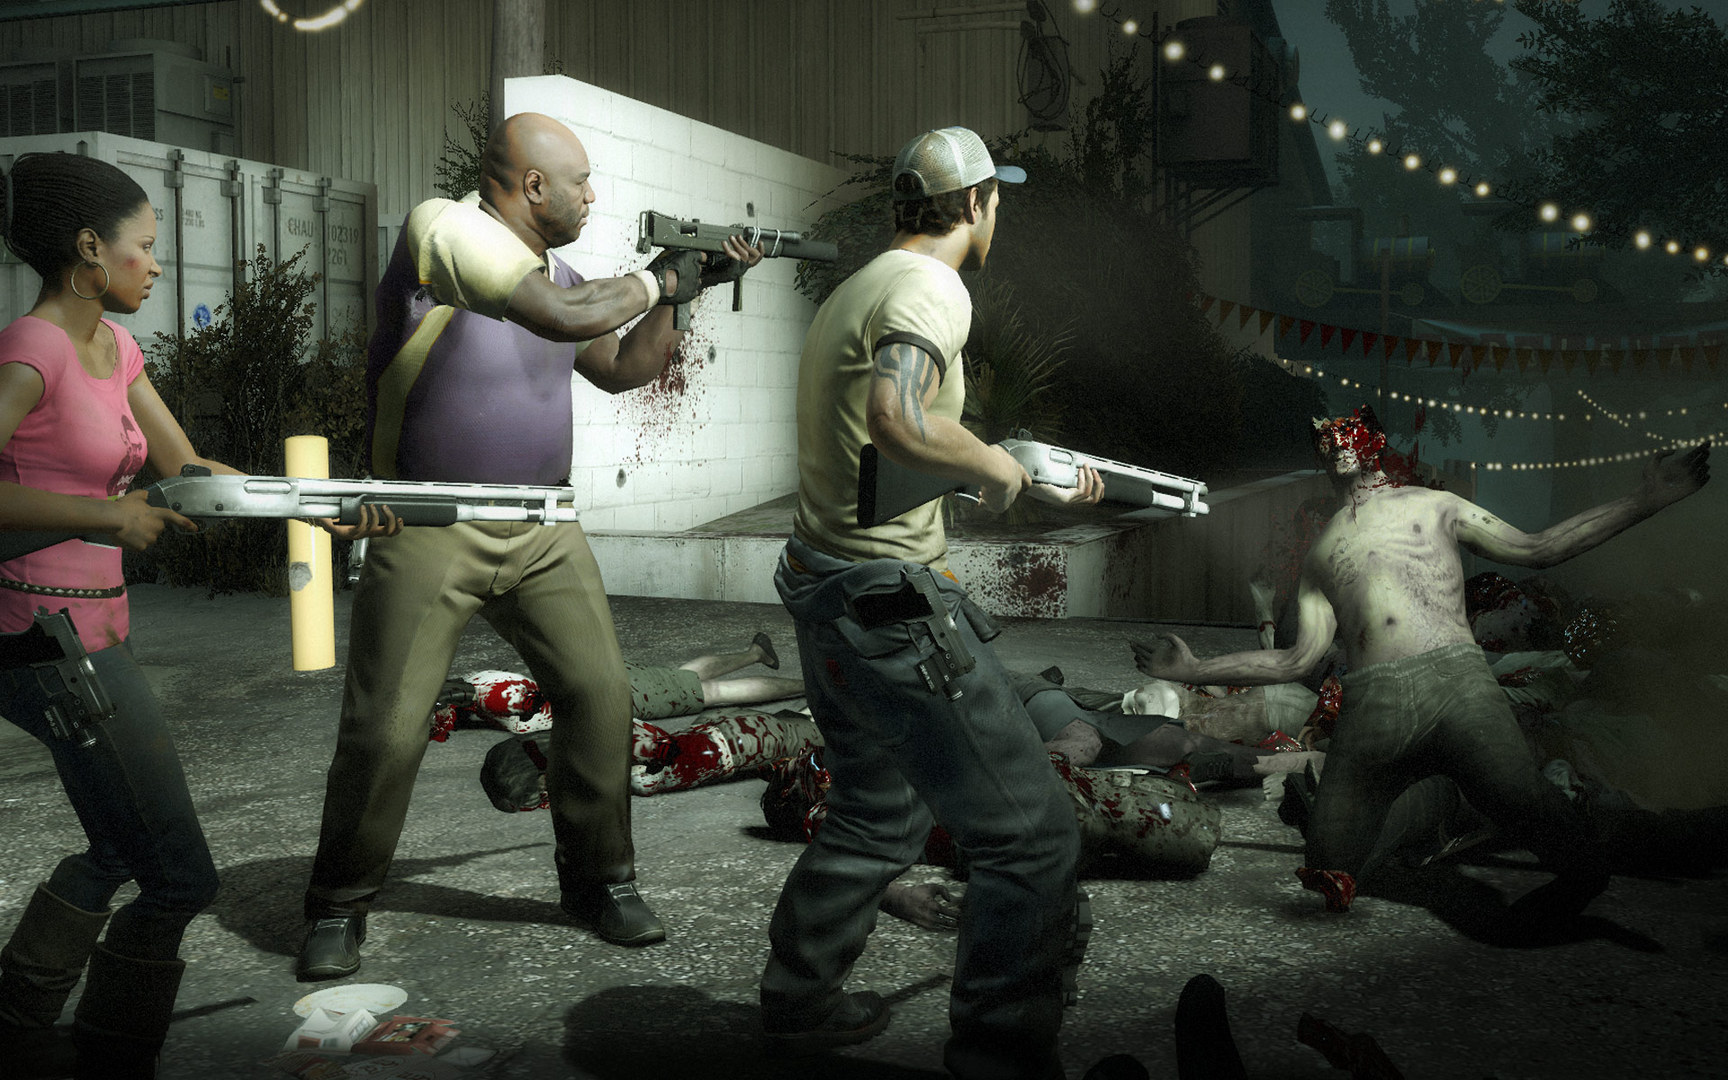
\includegraphics[width=\textwidth]{./img/l4d2.jpg}
  \end{center}
  \caption[ภาพเกม Left 4 Dead 2]{การเล่นแบบหลายผู้เล่นของเกม Left 4 Dead 2 ใช้การร่วมมือกันในการต่อสู้กับฝูงผีดิบ}
  \label{fig:L4D2}
\end{figure}
  

\subsection{Phasmophobia}

Phasmophobia เกมนี้ให้ผู้เล่นสวมบทบาทเป็นนักล่าผี และ รองรับผู้เล่นสูงสุด 4 คนที่ทำงานร่วมกันเพื่อสำรวจสถานที่และ รวบรวมหลักฐานเหตุการณ์เหนือธรรมชาติ โดยรวมแล้วเป็นเกมสยองขวัญที่ไม่เหมือนใครและน่าดึงดูด ซึ่งรวมเอาองค์ประกอบของการสืบสวน การเอาชีวิตรอด และการเล่นเกมแบบร่วมมือกัน เป็นเกมที่ต้องใช้การสื่อสาร การทำงานเป็นทีม และการคิดเชิงกลยุทธ์เพื่อให้ประสบความสำเร็จ \cite{Phasmophobia}

\begin{figure}[h]
  \begin{center}
  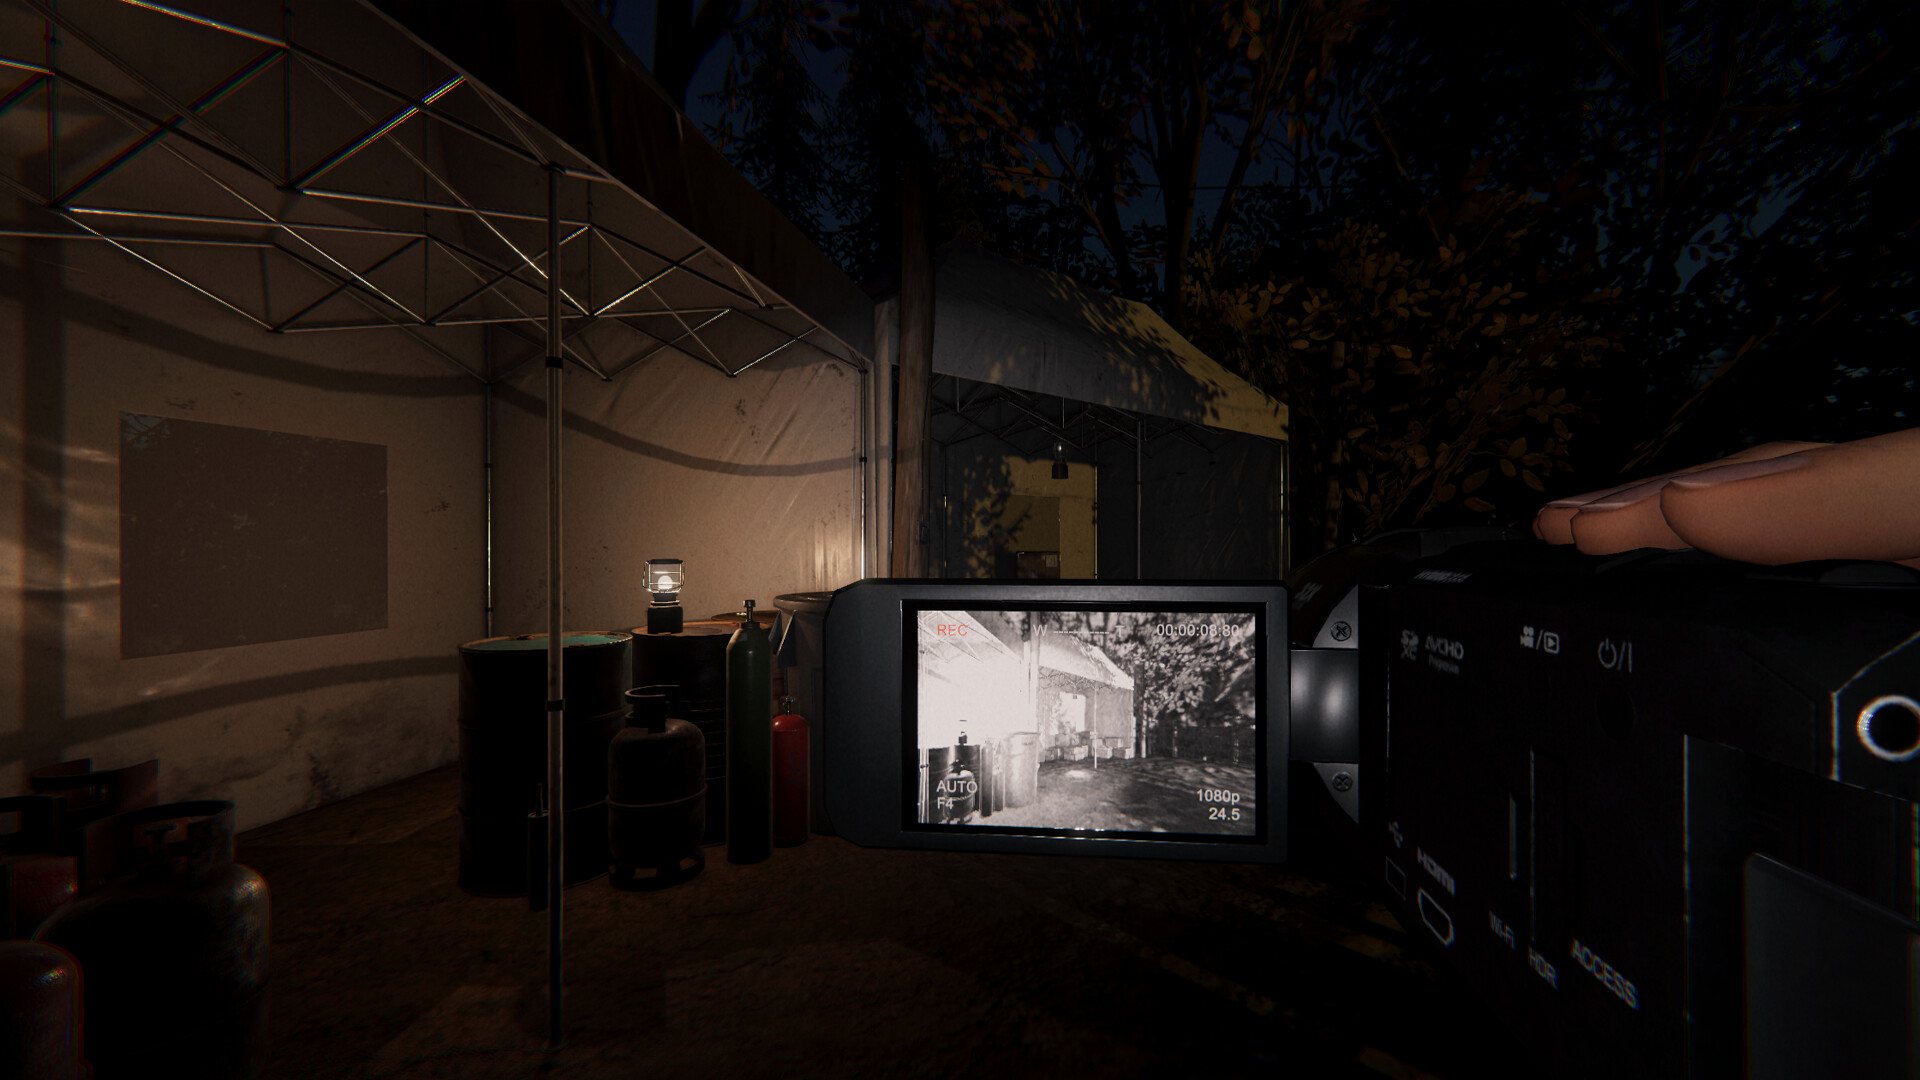
\includegraphics[width=\textwidth]{./img/phasmophobia.jpg}
  \end{center}
  \caption[ภาพเกม Phasmophobia]{การเล่นแบบหลายผู้เล่นของเกม Phasmophobia ใช้การร่วมมือกันในการสืบสวนเหตุการณ์เหนือธรรมชาติ เป็นเกมมุมมองบุคคลที่หนึ่ง}
  \label{fig:Phasmophobia}
\end{figure}
\subsection{The Forest}

The Forest เกมสยองขวัญเอาชีวิตรอด open world โดยผู้เล่นทำงานร่วมกันเพื่อสร้างที่พักพิง รวบรวมทรัพยากร และ ป้องกันมนุษย์กลายพันธุ์ โดยรวมแล้วเป็นเกมสยองขวัญเอาชีวิตรอดที่น่าตื่นเต้นและท้าทายที่นำเสนอการผสมผสานที่ไม่เหมือนใครระหว่างการสำรวจ การสร้าง และการต่อสู้ ด้วยบรรยากาศที่ตึงเครียด ศัตรูที่ท้าทาย และโลกที่สมจริง \cite{TheForest}

\begin{figure}[h]
  \begin{center}
  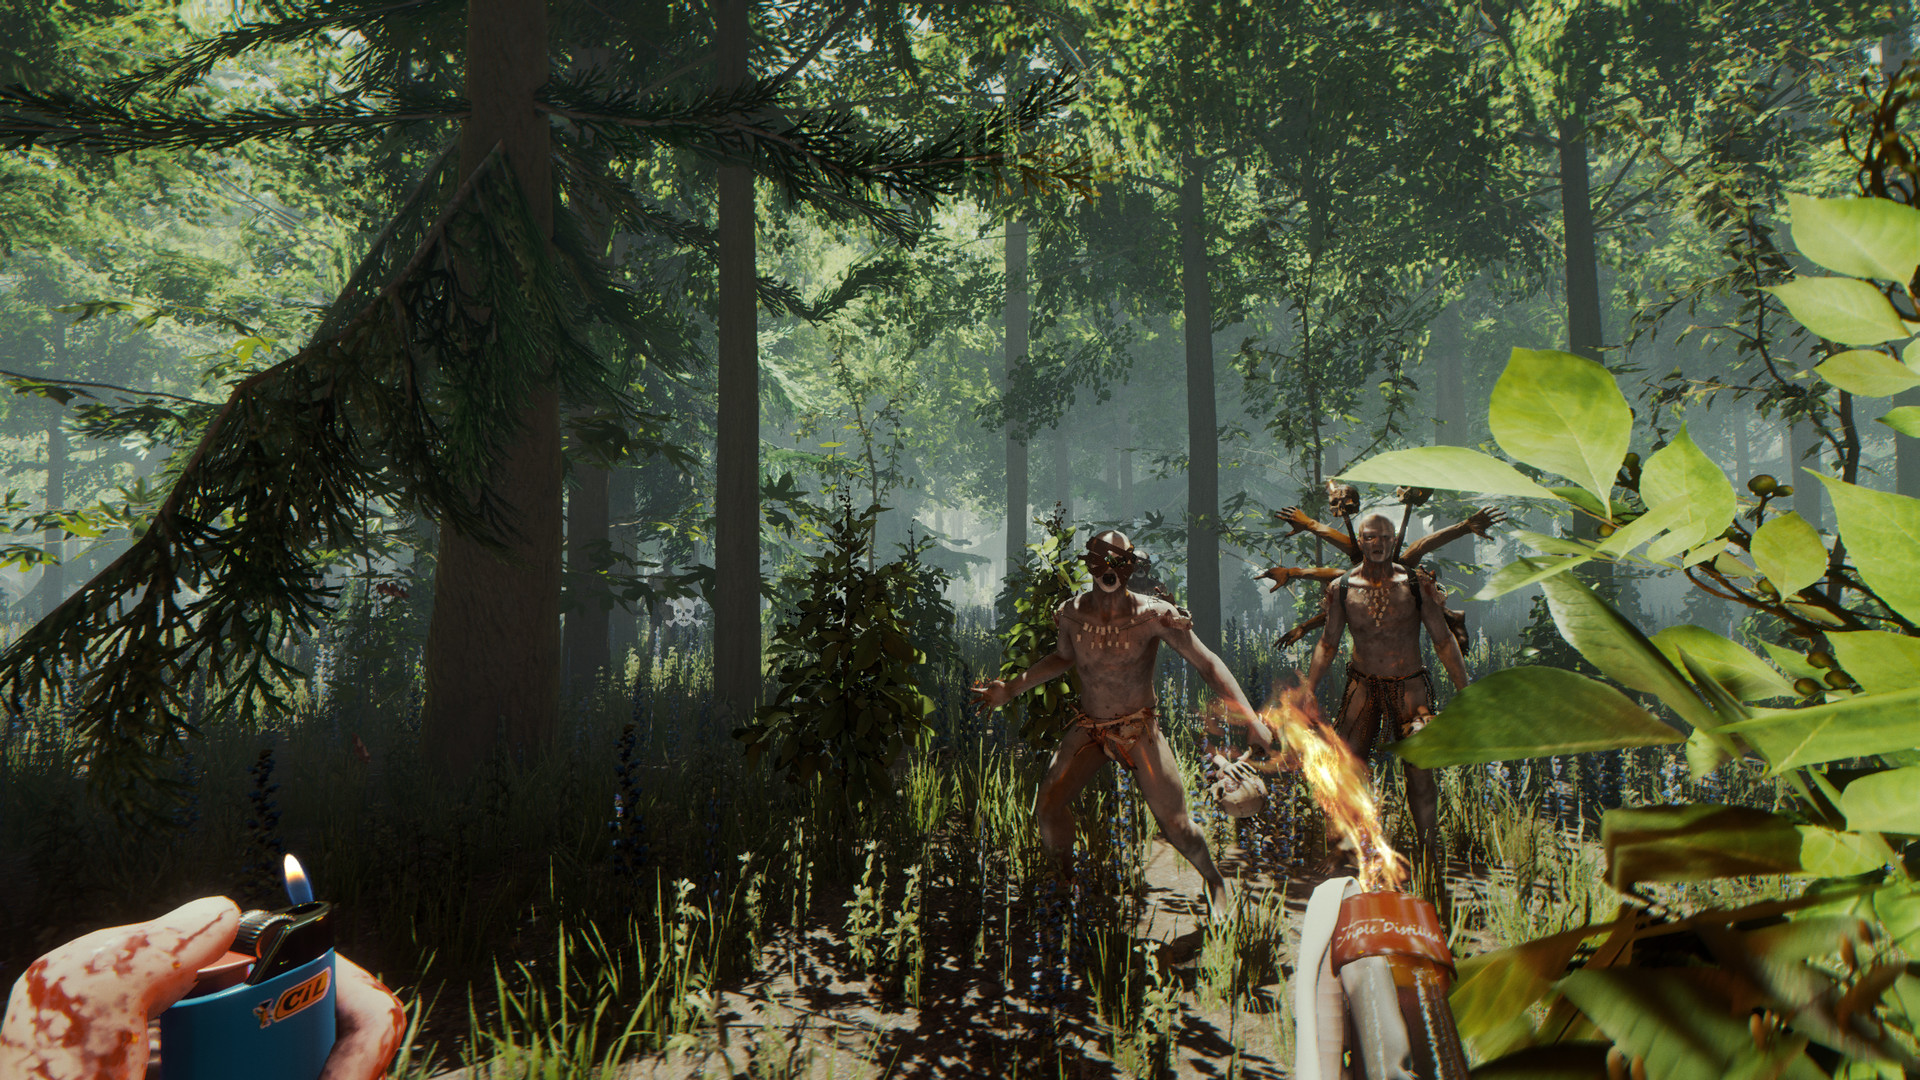
\includegraphics[width=\textwidth]{./img/theforest.jpg}
  \end{center}
  \caption[ภาพเกม The Forest]{เอาชีวิตรอดจากมนุษย์กลายพันธุ์กินคนในโลกเปิดของเกม The Forest}
  \label{fig:TheForest}
\end{figure}

\subsection{Devour}

Devour เป็นเกมสยองขวัญเอาชีวิตรอดแบบอาศัยความร่วมมือของผู้เล่น 1-4 คน แต่ละเกมยาวหนึ่งชั่วโมง หน้าที่ของผู้เล่น คือ ทำภารกิจในรูปแบบต่าง ๆ เพื่อเอาตัวรอดจากสมาชิกลัทธิที่ถูกผีสิง เช่น การเผาแพะเพื่อทำพิธีกรรม โดยผู้เล่นจะต้องรวบรวมทรัพยากรต่าง ๆ เพื่อใช้ในการทำภารกิจ และต้องระวังศัตรูที่อยู่รอบตัว \cite{Devour}

\begin{figure}[h]
  \begin{center}
  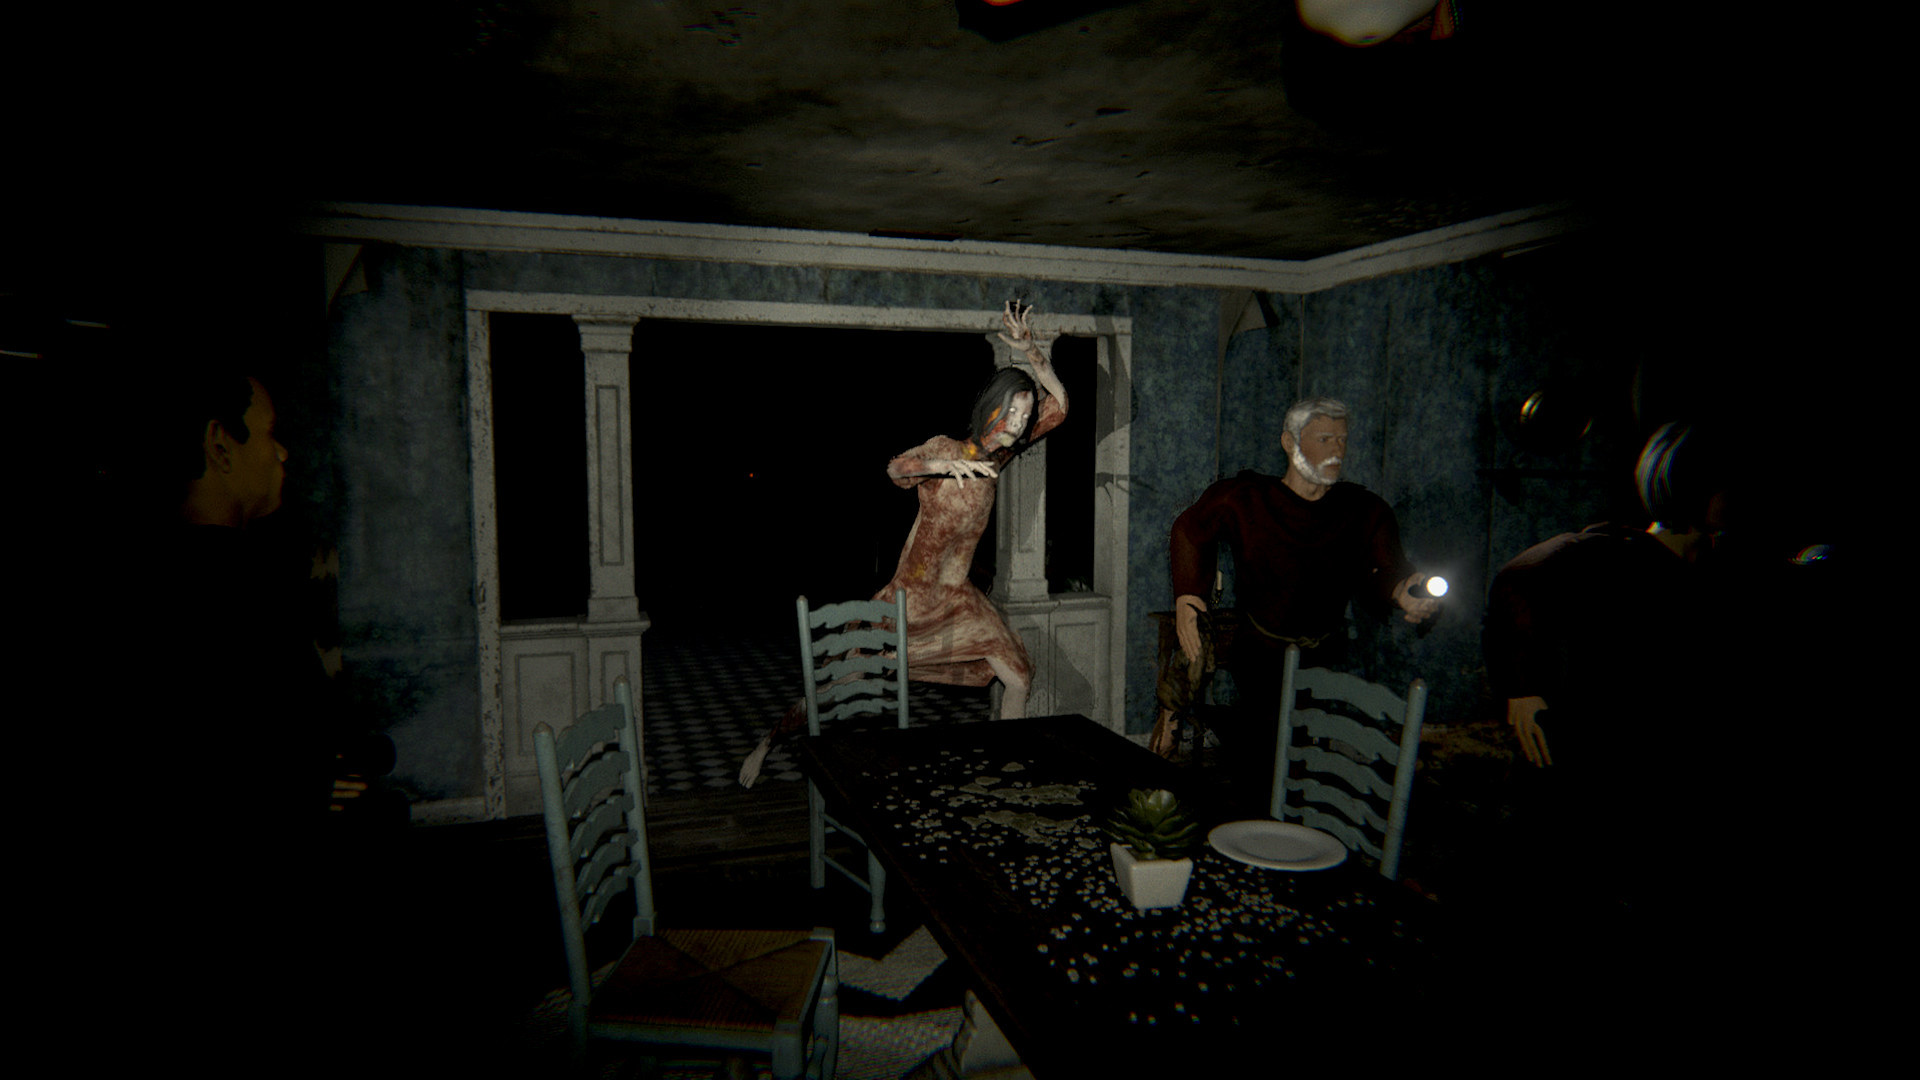
\includegraphics[width=\textwidth]{./img/devour.jpg}
  \end{center}
  \caption[ภาพเกม Devour]{ผู้เล่น 4 คน เอาชีวิตรอดจากสมาชิกลัทธิที่ถูกผีสิงในเกม Devour}
  \label{fig:Devour}
\end{figure}

\section{เทมเพลตการออกแบบเกม The Master Doc (Game Design Template Master Doc)}

การออกแบบเกมควรเป็น iterative process การเขียน documentation ที่มากเกินไป ทำให้การเปลี่ยนแปลงบางส่วนของเกมทำได้ยาก การออกแบบเกมควรเขียนเป็นแบบ high-level \cite{GDD2} เทมเพลต \cite{GDD1} นี้จะช่วยให้การออกแบบเกมง่ายขึ้น โดยมุ่งเน้นไปที่ความชัดเจนและจุดประสงค์ของแต่ละส่วนของเกมที่ถูกออกแบบมา โดยแบ่งออกเป็น 4 ส่วนใหญ่ ๆ

\subsection{ภาพรวมของเกม}
อธิบายให้เห็นถึงเกมอย่างคร่าวๆ และเน้นไปที่เกมที่เราจะพัฒนา โดยมีภาพประกอบเพื่อให้ให้เห็นภาพได้ชัดเจนมากขึ้น
\subsection{แนวคิดหลักของเกม}
อธิบายแนวคิดหลักของเกม โดยจะแบ่งออกเป็น 3 ส่วนได้แก่
\subsubsection{Design Pillar}
เขียนรากฐานของเกมและไม่ควรเปลี่ยนแปลง การออกแบบทั้งหมดควรเชื่อมโยงกับ design pillar เหล่านี้
\subsubsection{Game loop}
เขียนว่าเกมจะมีการเล่นอย่างไร และผู้เล่นจะทำอะไรในแต่ละรอบ
\subsubsection{การจูงใจผู้เล่น}
แรงจูงใจในการเล่นของผู้เล่นและ progression

\subsection{คุณสมบัติของเกม} 
ออกแบบคุณสมบัติในเกมของคุณ เป็นกลไกของเกมที่ใช้ตลอดทั้งเกม

\subsubsection{บริบท (Context)}
อธิบายเหตุผลที่ต้องมีคุณสมบัตินี้ และวิธีที่คุณสมบัตินี้ถูกออกแบบ
\subsubsection{สมมติฐาน (Hypothesis)}
อธิบายสิ่งที่คุณสมบัตินี้จะส่งผลกับผู้เล่น และวิธีที่คุณสมบัตินี้จะเชื่อมโยงกับแนวคิดหลักของเกม (Design Pillar)
\subsubsection{การวัดผลความสำเร็จ (Measuring success)}
อธิบายวิธีการวัดผลความสำเร็จของคุณสมบัตินี้ ไม่ว่าจะเป็นตัวชี้วัดหรือพฤติกรรมที่คาดหวังจากผู้เล่นตอน playtest
\subsubsection{การออกแบบ (Design)}
อธิบายวิธีการทำงานของคุณสมบัตินี้

\subsection{เนื้อหาของตัวเกม}
อธิบายเนื้อหาของตัวเกม หลัก ๆ ประกอบไปด้วย 3 ส่วนด้านล่าง ทั้งนี้ขึ้นอยู่กับประเภทของเกมที่เราจะพัฒนาด้วย

\begin{enumerate}
  \item สรุปเนื้อเรื่อง (Narrative Summary)
  \item ตัวละคร (Characters)
  \item ภาพรวมของฉาก (Level Summaries)
\end{enumerate}

\section{\ifenglish%
\ifcpe CPE \else ISNE \fi knowledge used, applied, or integrated in this project
\else%
ความรู้ตามหลักสูตรซึ่งถูกนำมาใช้หรือบูรณาการในโครงงาน
\fi
}

\begin{enumerate}
  \item Software Engineering: ใช้ความรู้เรื่องการจัดการการพัฒนาซอฟต์แวร์
  \item Computer Networking: ใช้ความรู้ในเรื่องเครือข่ายคอมพิวเตอร์ในการพัฒนาส่วนการเล่นหลายคน
  \item Object-oriented Programming: ใช้ความรู้ในการเขียนโปรแกรมเชิงวัตถุในการเขียนโปรแกรม
\end{enumerate}


\section{\ifenglish%
Extracurricular knowledge used, applied, or integrated in this project
\else%
ความรู้นอกหลักสูตรซึ่งถูกนำมาใช้หรือบูรณาการในโครงงาน
\fi
}


\begin{enumerate}
  \item การพัฒนาเกมด้วย Unreal Engine โดยใช้ Blueprint และภาษา C++
  \item การออกแบบวิธีการเล่นและฉาก
  \item การออกแบบงานศิลป์ในเกม
  \item การสร้างเนื้อเรื่องและเนื้อหาในเกม
\end{enumerate}
